\section{Auswertung}

\subsection{Symmetrische Drehstromlast }
\begin{enumerate}[label=\alph*)]
  \item Berechnen Sie unter Verwendung von Gleichung (7) für die Belastungen nach 3.3 (a) die komplexe Scheinleistung $\underline S$ aus den komplexen Größen $\underline U_{1N}$, $\underline U_{2N}$, $\underline U_{3N}$ sowie $\underline I_{1}$, $\underline I_{2}$, $\underline I_{3}$, und ermitteln Sie hieraus die von der Last aufgenommene Wirk- und die Blindleistung.
    \begin{align*}
      \underline S &= \underline U_{1N} \cdot \underline I_1^* + 
                      +\underline U_{2N} \cdot \underline I_2^*
                      +\underline U_{3N} \cdot \underline I_3^*\\
      \underline S &= 232Ve^{j0^\circ}\cdot 0,96Ae^{-(-j70^\circ)} + 234Ve^{j240^\circ}\cdot 0,9Ae^{-(j170^\circ)} + 233Ve^{j120^\circ}\cdot 0,2Ae^{-(j50^\circ)}\\ 
      \underline S &= 650,44 VA \cdot e^{j70^\circ} = 223.82 W + j614.93 Var\\
      P &= Re\{\underline S\} = 223.82 W \\
      Q &= Im\{\underline S\} = 614.93 Var
      % \underline U_{12}&= \underline U_{1N} - \underline U_{2N} = 232Ve^{j0} - 234Ve^{j240} = 403,6Ve^{j30,1^\circ}\\
      % \underline U_{23}&= \underline U_{2N} - \underline U_{3N} = 234Ve^{j240} - 233Ve^{j120} = 404,4Ve^{-j90,1^\circ}\\
      % \underline U_{31}&= \underline U_{3N} - \underline U_{1N} = 233Ve^{j120} - 232Ve^{j0} = 401,8Ve^{149,9^\circ}\\
      % \underline U_m &= \frac{U_{12} + U_{23} + U_{31}}{3}\\
      % \underline U_m &= \frac{403,6V+404,4V+401,8V}{3}\\
      % \underline I_m &= \frac{\underline I_{1} + \underline I_{2} + \underline I_{1}}{3}\\
      % \underline I_m &= \frac{}{3}\\
      % \underline S &= \sqrt 3 \cdot \underline U_m \cdot \underline I_m\\
    \end{align*}
		
	\item Bestimmen Sie für 3.3 (a) den Wirkleistungsfaktor $\cos\varphi$ der Last. Verwenden Sie hierfür die Ergebnisse aus (a). 
    \begin{align*}
      \underline S &= |S|\cdot e^{j\varphi} = 650,44 VA \cdot e^{j70^\circ}\\
      \Rightarrow \varphi &= 70^\circ
    \end{align*}
	
  \item Zeichnen Sie für die Belastungen nach 3.3 (a) das Zeigerdiagramm der Spannungen $\underline{U}_{1N}$, $\underline U_{2N}$, $\underline U_{3N}$ und $\underline U_{K}$ sowie das Zeigerdiagramm der Ströme $\underline I_{1}$, $\underline I_{2}$, $\underline I_{3}$ und $\underline I_{N}$.
		 		
	 		\begin{figure}[h!]
	 			\centering
	 			\begin{subfigure}[b]{0.5\textwidth}
	 				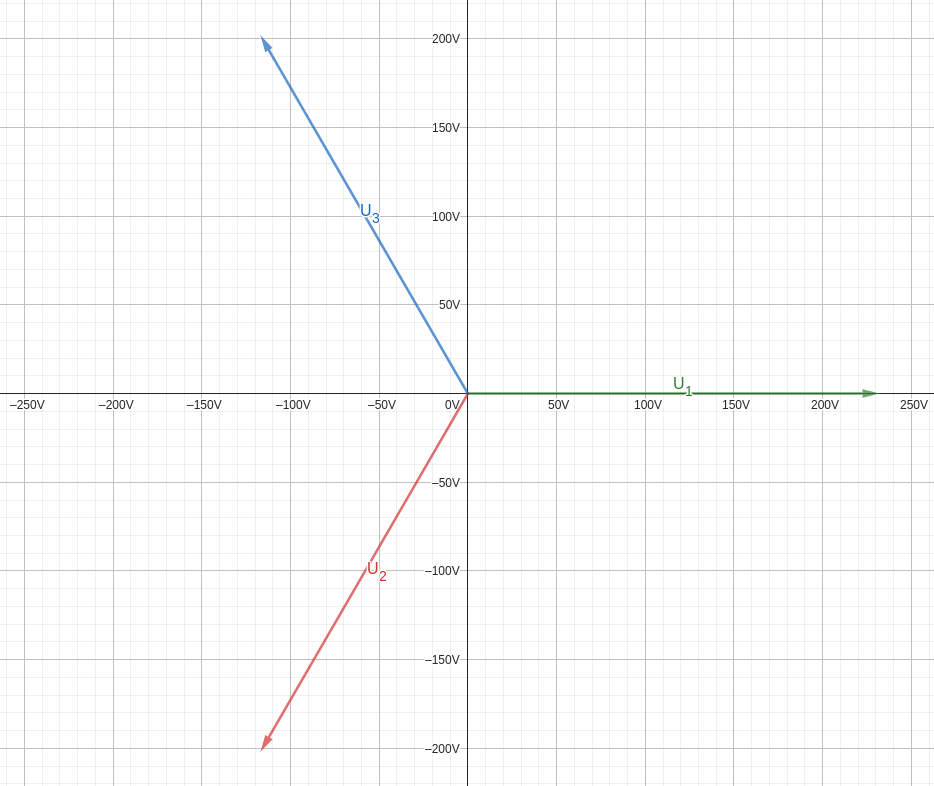
\includegraphics
	 				[width=\textwidth]{img/img3.3.2.png}
	 			\end{subfigure}\hfil
	 			\caption{Skizze der Spannungen - Symmetrische Drehstromlast ohne Kompensation}
	 		\end{figure}
      \pagebreak
	 			 		
	 		\begin{figure}[h!]
	 			\centering
	 			\begin{subfigure}[b]{0.5\textwidth}
	 				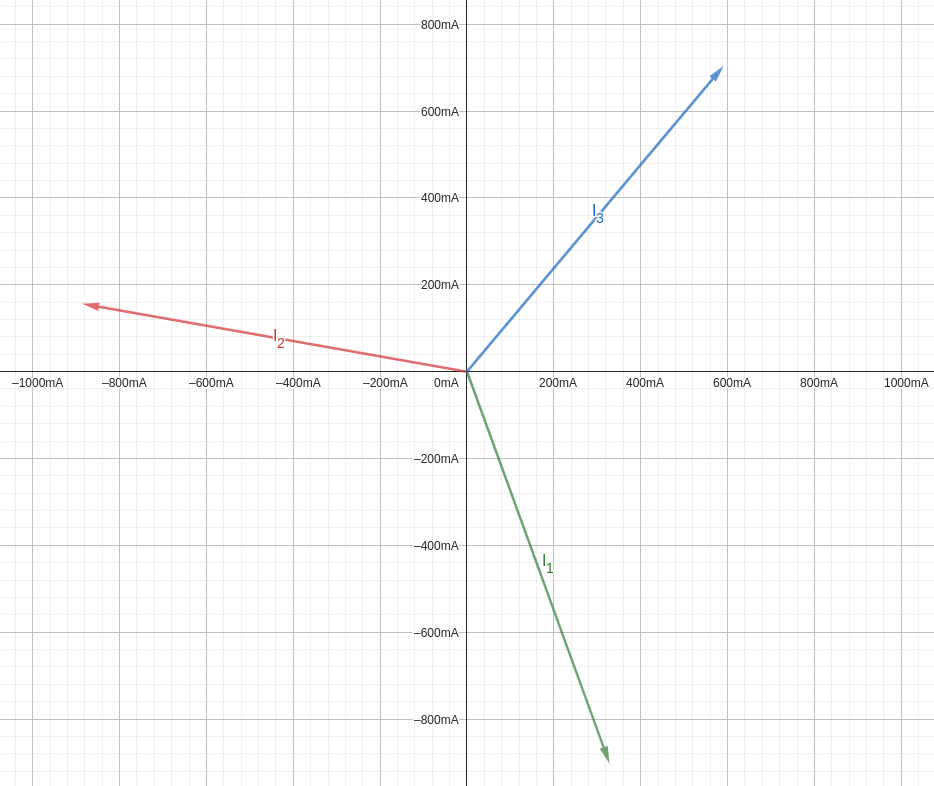
\includegraphics
	 				[width=\textwidth]{img/img3.3.3.png}
	 			\end{subfigure}\hfil
	 			\caption{Skizze der Ströme - Symmetrische Drehstromlast ohne Kompensation}
	 		\end{figure}

	\item Bewerten Sie Ihre Beobachtungen für 3.3 (b), (d) und (e) anhand der aufgenommenen Oszillogramme und Ihrer Versuchsvorbereitungen.
	\\
	
	\textbf{In Abschnitt 3.3 (b)} haben wir eine symmetrische Verbindung mit dem Knotenpunkt untersucht und festgestellt, dass die Strangströme im Vergleich zur Spannung eine Phasenverschiebung von 70° aufweisen. Beim Anschluss des Neutralleiters an diesen Knotenpunkt konnten wir keinen signifikanten Unterschied feststellen, da die Last symmetrisch ist.
	\\ \ \\
	\textbf{Im Abschnitt 3.3 (d)} haben wir die Spannungen und Ströme bei der Dreieckkompensation analysiert. Dabei bemerkten wir, dass die Strangströme im Vergleich zur Spannung keine Phasenverschiebung aufwiesen. Allerdings konnten wir Ober- und Unterschwingungen in den Strömen beobachten.
	\\ \ \\
	\textbf{Im Abschnitt 3.3 (e)} betrachteten wir die Stern-Kompensation und stellten fest, dass die Strangströme im Vergleich zur Spannung eine Phasenverschiebung von 70° aufwiesen. Es besteht die Gefahr, dass die Kompensation nicht wie erwartet funktioniert, da die Kondensatoren dennoch etwa dreimal größer sein sollten, um die Ergebnisse zu erzielen.
\end{enumerate}

\subsection{Unsymmetrische Drehstromlast }
\begin{enumerate}[label=\alph*)]
	\item Vergleichen Sie die gemessenen Werten unter 3.4 (a) und (b) mit den in der Vorbereitung errechneten Messwerten. Bewerten Sie die Unterschiede.
	 			\begin{table}[h!]
          \begin{center}
            \caption{Vergleich die gemessenen Werten unter 3.4 (a) mit den errechneten Messwerten}\label{tab:7}
	 				\begin{tabular}{r | c c | c c}
	 					\hline
            &\multicolumn{2}{c |}{\textbf{Messung}} &
            \multicolumn{2}{c }{\textbf{Rechnung}} \\
	 					\hline
            Art & \(\underline U_{eff}\ in\ V \) & \( Phase\ \varphi\ in\ ^\circ\ \ \)&
	 					\(\underline U_{eff}\ in\ V \) & \( Phase\ \varphi\ in\ ^\circ\ \ \)\\
	 					\hline
            $\underline U_{1N}$ & \( 234 \) & \( 0   \)  & \( 220 \) & \( 0   \) \\
	 					$\underline U_{2N}$ & \( 233 \) & \( 240 \)  & \( 220 \) & \( 240 \) \\
            $\underline U_{3N}$ & \( 233 \) & \( 120 \)  & \( 220 \) & \( 120 \) \\
            $\underline U_{KN}$ & \( 0   \) & \( 0   \)  & \( 0   \) & \( 0   \) \\
	 					\hline
            Art & \(\underline I_{eff}\ in\ mA \) & \( Phase\ in\ ^\circ\ \ \) &
	 					\(\underline I_{eff}\ in\ mA \) & \( Phase\ in\ ^\circ\ \ \) \\
	 					\hline
            $\underline I_{1}$	 & \( 140 \) & \( -22 \)  & \( 140 \) & \( -17,77 \)\\
            $\underline I_{2}$	 & \( 116 \) & \( 240 \)  & \( 109 \) & \( 240 \)\\
	 					$\underline I_{3}$	 & \( 84  \) & \( 156 \)  & \( 81  \) & \( 156 \)\\
	 					$\underline I_{N}$	 & \( 114 \) & \( 90  \)  & \( 114 \) & \( 93  \)\\
	 					\hline
	 				\end{tabular}
	 		\end{center}
    \end{table}

      \pagebreak
      \begin{table}[h!]
        \begin{center}
          \caption{Vergleich die gemessenen Werten unter 3.4 (b) mit den errechneten Messwerten}\label{tab:8}
	 				\begin{tabular}{r | c c | c c}
	 					\hline
            &\multicolumn{2}{c |}{\textbf{Messung}} &
            \multicolumn{2}{c }{\textbf{Rechnung}} \\
	 					\hline
	 					Art & \(\underline U_{eff}\ in\ V \) & \( Phase\ \varphi\ in\ ^\circ\ \ \)  &
	 					\(\underline U_{eff}\ in\ V \) & \( Phase\ \varphi\ in\ ^\circ\ \ \)  \\
	 					\hline
	 					$\underline U_{1N}$ & \( 234 \) & \( 0   \) & \( 220 \) & \( 0   \) \\
	 					$\underline U_{2N}$ & \( 231 \) & \( 239 \) & \( 220 \) & \( 240 \) \\
            $\underline U_{3N}$ & \( 233 \) & \( 119 \) & \( 220 \) & \( 120 \) \\
            $\underline U_{KN}$ & \( 82  \) & \( 268 \) & \( 75  \) & \( 273 \) \\
	 					\hline
            Art & \(\underline I_{eff}\ in\ mA \) & \( Phase\ in\ ^\circ\ \ \)&
	 					\(\underline I_{eff}\ in\ mA \) & \( Phase\ in\ ^\circ\ \ \) \\
	 					\hline
            $\underline I_{1}$	 & \( 150 \) & \( 3   \) & \( 148 \) & \( 1,3   \) \\
	 					$\underline I_{2}$	 & \(  81 \) & \( 228 \) & \(  81 \) & \( 225 \) \\
	 					$\underline I_{3}$	 & \( 112 \) & \( 148 \) & \( 107 \) & \( 149 \) \\
	 					$\underline I_{N}$	 & \( 0   \) & \( 0   \) & \( 0   \) & \( 0   \) \\
	 					\hline
	 				\end{tabular}
	 		\end{center}
\end{table}
	
      Die Tabelle \ref{tab:7} und \ref{tab:8} zeigt, dass die gemessenen Spannungen und Ströme äquivalent zu den rechnerisch ermittelten Werten sind.  Die Ströme weisen geringfügige Abweichungen von den Messwerten auf, die jedoch als vernachlässigbar angesehen werden können.

Bei der Rechnung wurde angenommen, dass die Strangspannung 220 V beträgt, wobei die gemessenen Werte der Standardnetzspannung von 230 V entsprechen.
	\item Berechnen Sie die komplexe Scheinleistung $\underline S$, und ermitteln Sie hieraus die Wirk- und die Blindleistung (dreiphasig) für die unter 3.4 gemessenen Drehstromlast
    \begin{align*}
      \underline S &= \underline U_{1N} \cdot \underline I_1^* + 
                      +\underline U_{2N} \cdot \underline I_2^*
                      +\underline U_{3N} \cdot \underline I_3^*\\
      \underline S &= 234Ve^{j0^\circ}\cdot 0,15Ae^{-(j3^\circ)} + 231Ve^{j239^\circ}\cdot 0,08Ae^{-(j228^\circ)} + 233Ve^{j119^\circ}\cdot 0,11Ae^{-(j148^\circ)}\\ 
      \underline S &=76,37 VA \cdot e^{-j8,08^\circ} = 75,61 W -j 10,74 Var\\
      P &= Re\{\underline S\} = 75,61 W \\
      Q &= Im\{\underline S\} = -10,74 Var
    \end{align*}

\end{enumerate}
